\documentclass{article}
\usepackage[utf8]{inputenc}


\usepackage{enumerate}
\usepackage{amsmath} % Tillater avansert formatering av matte.
\usepackage{amsfonts} % Tillater avanserte teikn, som R for reelle tall.
\usepackage{graphicx} % Tillater mer avansert formatering av grafikk.
\usepackage{geometry} % Tillater enklere formatering av sidevisning.
\usepackage{physics}
\usepackage{amssymb}
\setlength\parindent{0pt}

\title{Project 1}
\author{Johanne Mehren, Stine Sagen and Marit Kollstuen}


\begin{document}


\begin{abstract}
We present our Ferrari algorithm for solving linear equations. Our best algorithm runs as $4n$ FLOPS with $n$ the dimensionality of the matrix.
\end{abstract}


\maketitle

\section{Introduction}
The main goal of project 1 is to understand the concept of dynamic memory allocation, a memory handling frequently used in programs such as C++ and Fortran. In C++ you have three ways of managing memory; statically, locally or dynamically. By using dynamic memory allocation, we are reserving space for saving data and are able to manage the lifetime of allocated memory. 

\section{Theory, algorithms and methods}
\subsection{Exact solution}
The one-dimensional Poisson equation \begin{equation} -u''(x) = f(x) \end{equation} does have an exact (analytical) solution of the form: \begin{equation} u(x) = 1 - (1-e^{-10})x - e^{-10x} \end{equation} when assuming the source term on the right hand side of the Poisson equation is \begin{equation} f(x) = 100e^{-10x}. \end{equation} Substituting the above solution into our differential equation, we can then verify that this turns out to be correct. 

\begin{align*}
u(x)& = 1 - (1-e^{-10})x - e^{-10x}  \\
u'(x)& = -1 + e^{-10} + 10e^{-10x} \\
u''(x)& = -100e^{-10x}  \\
-(-100e^{-10x})& = 100e^{-10x} \\
\therefore \\
100e^{-10x}& = 100e^{-10x}
\end{align*}

As expected, $u(x) = 1 - (1-e^{-10})x - e^{-10x}$ is an exact solution of $-u''(x) = f(x)$ .\\

Our differential equation conserns a boundary value problem which means our solution also needs to satisfy the given boundary conditions. 

Checking the behavior of the exact solution at its bondary points 0 and 1: 

\begin{align*}
u(0)& = 1-(1-e^{-10})\cdot 0 -e^{-10\cdot 0} = 0 \\
u(1)& = 1-(1-e^{-10})\cdot 1 -e^{-10\cdot 1} = 0 \\
\end{align*}

$u(x) = 1 - (1-e^{-10})x - e^{-10x}$ is indeed a solution of our boundary value problem. 
\\\\
In our project we want to compare this exact solution with the numerical solution we obtain when the boundary value problem takes a discretized form. 

\subsection{Finite difference method}

We want to solve the Poisson equation numerically and this can be achived by something we call finite-difference methods. Finite-difference methods are about replacing the derivatives appearing in the differential equation by finite difference approximations at a given set of discrete points in space and/or time. E.g when this method is applied to the second order derivative in the poisson equation, we obtain a dicretized approximation for u in the x-direction because its only depended on the x variable. In deriving these finite difference approximations, Taylor series expansion might be very useful.

\subsubsection{Taylor series expansion}

We might use Taylor series expansion in order to derive a suitable finite difference approximation for the differential equation in the process for obtaining a numerical solution. 
\\
Assuming our function u(x) is higher order differensible we can preform a Taylor expansion forward and backward in space:
\begin{align*}
u(x+h)& = u(x) + hu' + \frac{h^2u''}{2!}  + \frac{h^3u'''}{3!} + o(h^4) \\ 
u(x-h)& = u(x) - hu' +  \frac{h^2u''}{2!} -\frac{h^3u'''}{3!} + o(h^4)
\intertext{To obtain finite difference approximation for the second order derivative we then sum the two equations:}
u(x+h) + u(x-h)& = 2u(x) + \frac{2h^2u''}{2!} + o(h^4) \\
\intertext{In the end we solve for  $u'' $ and get:}
u'&' = \frac{u(x+h) + u(x-h) -2u(x)}{h^2} + o(h^2) \\
\end{align*}

\subsubsection{Discretization of the bondary value problem}

As already mentioned the concept of discretizing is about dividing the domain into a finite set of discrete points. We now the discretize $u$ as $v_i$ with grid points $x_i =  ih$  in the range from $x_0= 0$ to $x_{n+1}=1$. The grid spacing is defined as $h = \frac{x_{n+1}-x_0}{n+1} = \frac{1-0}{n+1} = \frac{1}{n+1}$. The boundary conditions are $v_0 = v_{n+1} = 0$. Our approximated finite difference approximation for the poisson equation is now:

\begin{equation} 
-\frac{v_{i+1} + v_{i-1} -2v_i}{h^2} 
\end{equation}



\subsection{A general algorithm for solving the tridiagonal matrix}
\subsection{Specialized algorithm for solving the tridiagonal matrix}
\subsection{Relative error}

\begin{equation}
	\epsilon_i = log_{10}(\abs{\frac{v_i -u_i}{u_i}})
	\label{eq:re}
\end{equation}

\subsection{LU-decomposition}



\section{Project 1 a)}

We are attempting to solve the equation: 

\begin{align*}
	-u''(x) & = f(x), x \in (0, 1), u(0) = u(1) = 0
\end{align*}

which can be approximated as:

\begin{equation}
	v_i" \approx -\frac{v_{i-1}- 2v_i + v_{i+1}}{h^2}
\end{equation}

Assumed $n= 4$, it can be shown that this can be represented as a Toepliz-matrix by setting: 

\[
\begin{bmatrix}
	v
\end{bmatrix}
=
\begin{bmatrix}
	 v_1 & v_2 & v_3 & v_4
\end{bmatrix}
\]

For which 

\[
\begin{bmatrix}
	v_1" \\  v_2" \\ v_3" \\ v_4"
\end{bmatrix}
	\approx -\frac{1}{h^2}
\begin{bmatrix}
	-(v_{0} -2v_1 +v_2) \\
	-(v_1 -2v_2 +v_3) \\
	-(v_{2} -2v_3 +v_4) \\
	-(v_{3} -2v_4 +v_5) 
\end{bmatrix}
\]

The boundary conditions are set to $v_0 = v_{n+1} = 0$, so the expression becomes: 

\[
\begin{bmatrix}
	2 & -1 & 0 & 0 \\
	-1 & 2 & -1 & 0 \\
	0 & -1 & 2 & -1 \\
	0 & 0 & -1 & 2
\end{bmatrix}
\begin{bmatrix}
	v_1 \\  v_2 \\ v_3 \\ v_4
\end{bmatrix}
	= -h^2
\begin{bmatrix}
	f_1 \\
	f_2 \\
	f_3 \\
	f_4
\end{bmatrix}
\]

In which $f_i$ is known. 

\section{Project 1 b)}

\begin{figure}[h]
    \centering
    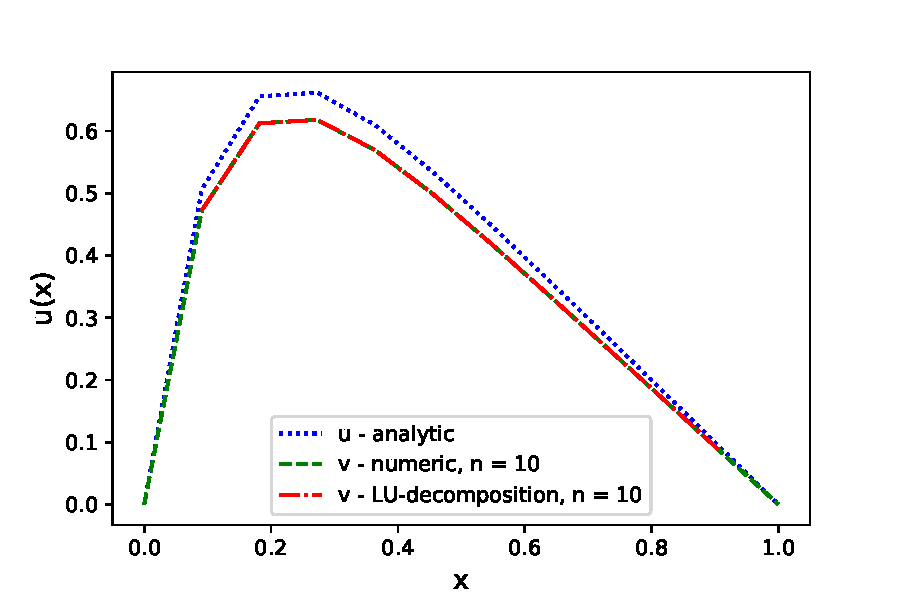
\includegraphics[width =12cm]{python/size_10.pdf}
    \caption{Size 10}
    \label{fig:1}
\end{figure}

\begin{figure}[h]
    \centering
    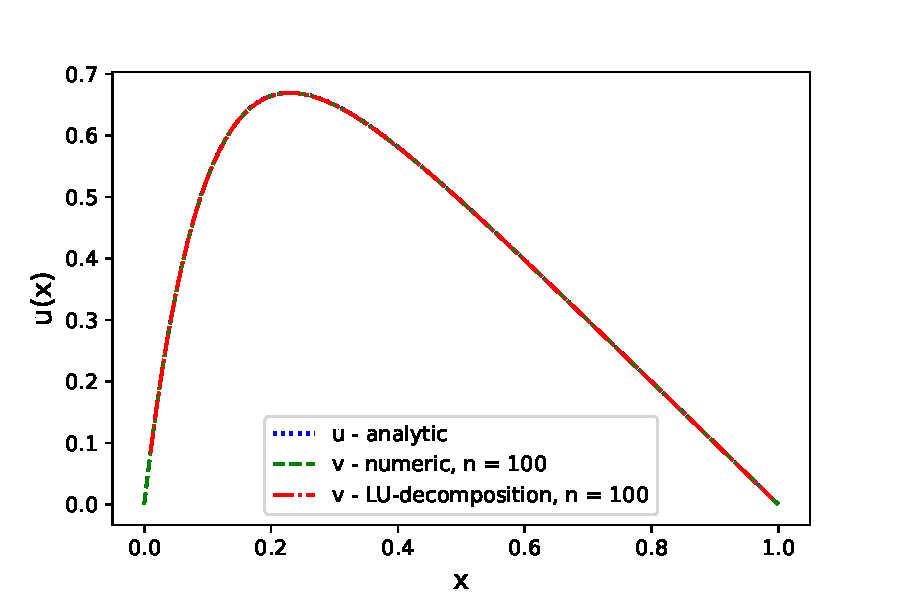
\includegraphics[width =12cm]{python/size_100.pdf}
    \caption{Size 100}
    \label{fig:2}
\end{figure}


\begin{figure}[h]
    \centering
    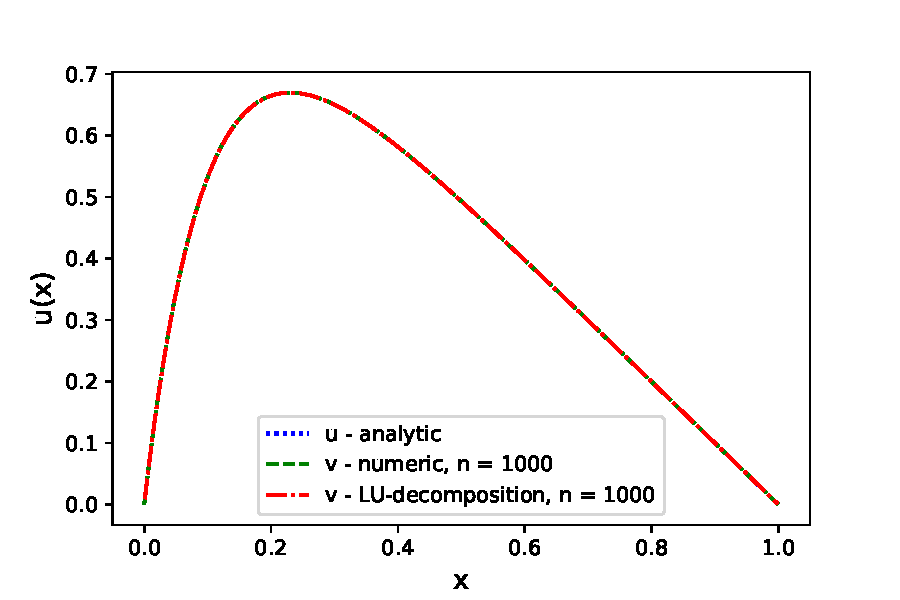
\includegraphics[width =12cm]{python/size_1000.pdf}
    \caption{Size 1000}
    \label{fig:3}
\end{figure}


\begin{figure}[h]
    \centering
    \includegraphics[width =12cm]{python/size_10000.pdf}
    \caption{Size 10000}
    \label{fig:4}
\end{figure}

\begin{figure}[h]
    \centering
    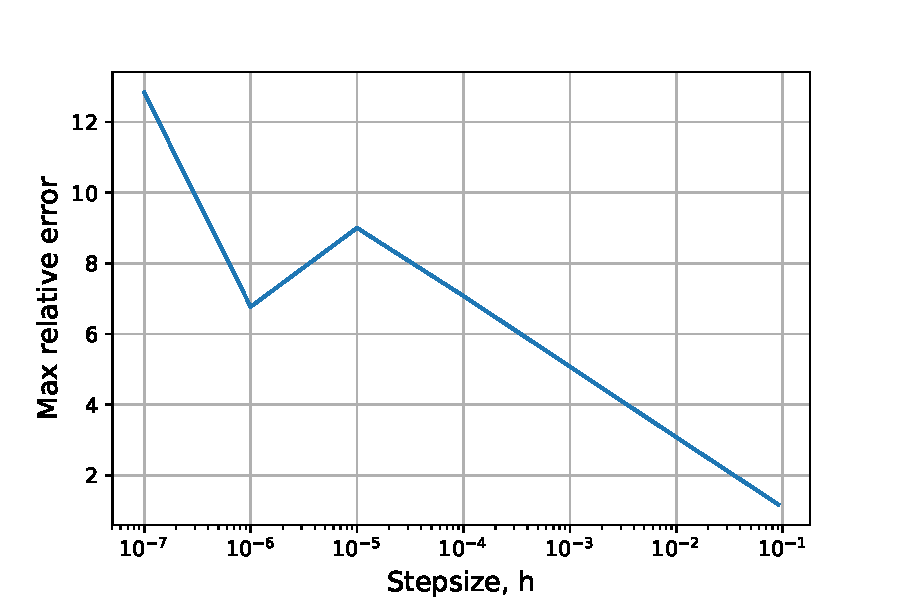
\includegraphics[width =12cm]{python/relative_error.pdf}
    \caption{Relative error}
    \label{fig:re}
\end{figure}

\begin{table}[]
\begin{tabular}{llll}
           & \multicolumn{3}{c}{\textbf{Time (s):}}                                                                  \\ \hline
           & \textbf{Gaussian elimination (g.a.):} & \textbf{Gaussian elimination (s.a.):} & \textbf{LU-decomposition:} \\ \hline
n = $10$   & $4.816e-05$                              & $4.196e-05$                              & $0.0001301$       \\
n = $10^2$  & $0.0003078$                              & $0.0002770$                              & $0.0002670$       \\
n = $10^3$ & $0.003332$                               & $0.003214$                               & $0.02403$         \\
n = $10^4$ & $0.03234$                                & $0.03215$                                & $14.26$           \\
n = $10^5$ & $0.3629$                                 & $0.3458$                                 & N/A               \\
n = $10^6$ & $3.109$                                  & $3.136$                                  & N/A               \\
n = $10^7$ & $32.79$                                  & $32.20$                                  & N/A              
\end{tabular}
\label{tab:1}
\caption{CPU-time for the different algorithms (g.a. = general algorithm, s.a. = special algorithm)}
\end{table}

\begin{table}[]
\centering
\begin{tabular}{ll}
\multicolumn{2}{c}{\textbf{Max. relative error, $\epsilon_{max}$:}} \\ \hline
n = $10$                                  & $1.1797$                                \\
n = $10^2$                                & $3.08804$                               \\
n = $10^3$                                & $5.08005$                               \\
n = $10^4$                                & $7.07936$                               \\
n = $10^5$                                & $9.0049$                                \\
n = $10^6$                                & $6.77137$                               \\
n = $10^7$                                & $12.8336$                              
\end{tabular}
\label{tab:2}
\caption{Relative error for the special algorithm using Equation \ref{eq:re}}
\end{table}


\section{Project 1 c)}
In this task we implement matrix 

\section{Project 1 d)}

\section{Project 1 e)}


\section{Conclusion}

\section{References}


\end{document}